\documentclass[10pt]{article}
\usepackage[polish]{babel}
\usepackage[utf8]{inputenc}
\usepackage[T1]{fontenc}
\usepackage{graphicx}
\usepackage[export]{adjustbox}
\graphicspath{ {./images/} }
\usepackage{amsmath}
\usepackage{amsfonts}
\usepackage{amssymb}
\usepackage[version=4]{mhchem}
\usepackage{stmaryrd}

\title{Zestaw 1. }

\author{}
\date{}


\begin{document}
\maketitle
\begin{center}

\includegraphics[max width=\textwidth]{2024_11_21_ba1800e73998f6feb233g-1(2)}
\end{center}

\section*{GIMNAZJUM}
\begin{enumerate}
  \item Dokładnie \(60 \%\) uczniów pewnego gimnazjum spędziło wakacje w górach, a dokładnie \(\frac{1}{3}\) uczniów tej szkoły - nad morzem. Ponadto dokładnie \(\frac{1}{15}\) pozostałych uczniów spędziła wakacje za granicą. Jaka jest najmniejsza liczba uczniów tego gimnazjum?. Odpowiedź uzasadnij.
  \item W drodze do domu Piotr postanowił zatankować, przez co czas jego podróży wydłużył się o \(10 \%\). Kolejnego dnia, przemierzając tę samą drogę, Piotr tankował dwa razy dłużej, przez co całkowity czas jego podróży wyniósł jedną godzinę. Ile czasu zajęłaby podróż Piotrowi, gdyby nie tankował?
  \item W trapezie \(A B C D\), w którym \(A D \| B C\), zachodzą równości \(|A B|=|B C|,|A C|=|C D|\)\\
oraz \(|B C|+|C D|=|A D|\). Wyznacz kąty tego trapezu.\\
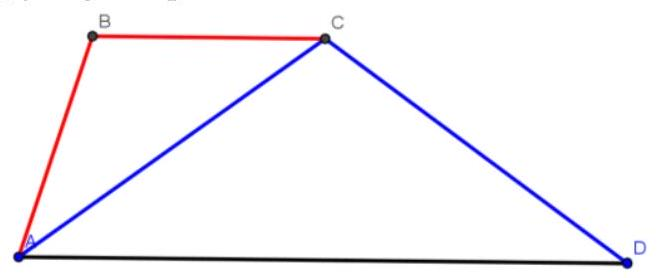
\includegraphics[max width=\textwidth, center]{2024_11_21_ba1800e73998f6feb233g-1(1)}
\end{enumerate}

\section*{LICEUM}
\begin{enumerate}
  \item W trójkącie \(A B C\) punkty \(K, L, M\) są spodkami wysokości opuszczonych odpowiednio z wierzchołków \(A, B\), \(C\). Udowodnij, że proste zawierające wysokości trójkąta \(A B C\) zawierają dwusieczne kątów wewnętrznych trójkąta KLM.\\
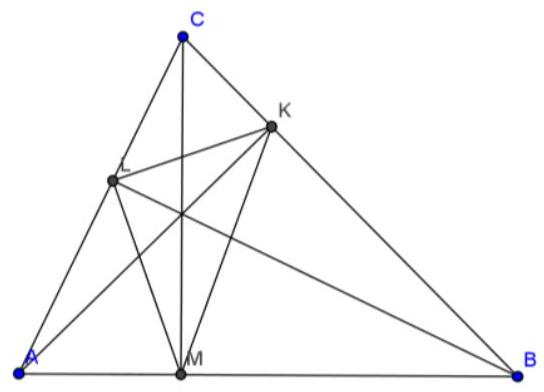
\includegraphics[max width=\textwidth, center]{2024_11_21_ba1800e73998f6feb233g-1}
  \item Czy istnieją takie liczby niewymierne \(x, y\), że
\end{enumerate}

\[
x+y=x y
\]

oraz liczba \(x+y=x y\) jest wymierna? Odpowiedź uzasadnij.\\
3. Udowodnij, że jeżeli suma wszystkich dzielników pewnej liczby naturalnej jest dwa razy większa od tej liczby, to suma odwrotności tych dzielników wynosi 2.

Rozwiązania należy oddać do piątku 16 stycznia do godziny 12.30 koordynatorowi konkursu panu Jarostawowi Szczepaniakowi lub swojemu nauczycielowi matematyki.

Nie trzeba rozwiąywać wszystkich zadań.


\end{document}